\documentclass[a4paper,10pt]{article}

\usepackage[boxruled,vlined,english]{algorithm2e}
\usepackage[francais,english]{babel}
\usepackage[utf8x]{inputenc}
\usepackage[T1]{fontenc}
\usepackage{graphicx}
\usepackage{hyperref}
\usepackage{latexsym}
\usepackage{setspace}
\usepackage{amsmath}
\usepackage{amssymb}
\usepackage{bookman}
\usepackage{amsthm}
\usepackage{amscd}
\usepackage{color}
\usepackage{calc}

\setlength{\voffset}{-3.75cm}
\setlength{\hoffset}{-2.6cm}
\setlength{\oddsidemargin}{2.75cm}
\setlength{\topmargin}{2in}
\setlength{\headheight}{0in}
\setlength{\headsep}{0in}
\setlength{\topskip}{0in}
\setlength{\parindent}{0cm}
\setlength{\parskip}{1ex plus0.4ex minus0.2ex}
\setlength{\textwidth}{16.25cm}
\setlength{\textheight}{21cm}
\renewcommand{\baselinestretch}{1.5}
\flushbottom
\setcounter{page}{1}
\setcounter{tocdepth}{2}

\SetKw{Edb}{Side effect}
\SetKw{Et}{and}
\SetKw{Ou}{or}
\SetKw{De}{from}
\SetKw{A}{to}
\SetKw{Par}{by}
\SetKwBlock{Debut}{Begin}{End}
\SetKwIF{Si}{SinonSi}{Sinon}{If}{then}{Else if}{Else}{EndIf}
\SetKwFor{Pour}{For}{do}{EndFor}
\SetKwFor{PourTout}{For all}{do}{EndFor}
\SetKwFor{TantQue}{While}{do}{EndWhile}
\SetKw{Retour}{Return}

\newcommand{\guill}[1]{``#1''}
\newcommand{\bigO}[1]{\mathcal O\left( #1 \right)}
\newcommand{\bigOmega}[1]{\Omega\left( #1 \right)}
\newcommand{\bigTheta}[1]{\Theta\left( #1 \right)}

\newtheorem{prob}{Problem}


% ??? Faire une Titlepage un peu plus jolie...
\title{ \Large Internship report \\ \LARGE TITRE???}

\author{\normalsize Romain \textsc{Versaevel}, M1 Informatique Fondamentale, ENS de Lyon \\ \normalsize Tutored by David \textsc{Meredith}, Associate professor at Aalborg University\\}

\date{\today}

\begin{document}

\maketitle

\begin{abstract}
\end{abstract}

\newpage
\tableofcontents
\newpage


\section{Introduction}

This report was written as part of a twelve-week internship I did during the summer 2015, as part of my Master 1 of Computer Sciences at ENS Lyon. This Internship took place at Aalborg University, Denmark, in the Department of Architecture, Design and Media Technology. I was supervised by Pr. David Meredith, who is Associate Professor there and specializes in Computer music.

The topic of this internship was to ???


%Le sujet de ce stage était d'analyser l'algorithme d'alignement multilingue \anym, conçu et implémenté par Adrien Lardilleux en 2009, disponible sur \cite{anymalign}, et utilisé par le LIMSI pour diverses applications.

%Ce rapport est divisé en quatre parties. Dans la première, je présente le contexte dans lequel s'inscrit mon travail, le domaine de la traduction automatique. Dans la deuxième, je présente l'algorithme que j'ai étudié et l'analyse qui en avait déjà été réalisée. Dans les troisième et quatrième, je présente les résultats de ma propre analyse, empirique (confrontation avec des mesures d'association) et théorique.
The report has two main sections. The first one consists in an introduction to the field of research, \emph{Computer music}, including ???
The second describes my work on ??? and its results. It is completed by a shorter section showing possible improvements and unrelated work I did.

\section{Computer music}

This section presents the area of \emph{Computer music}. It actually gives an overview of the ???
before focusing on 


\subsection{Short presentation, history, research areas}

The term \emph{Computer music} simply describes any activity that implies both music and computing tools.

Music and mathematics have been linked from the origins; the basis of western music was developed by the Pythagoreans in the 5th century BCE; the French composer Jean-Philippe Rameau used mathematical tools to theorise harmony in the 18th century, in \cite{rameau} for example. Sound is a physical vibration, and has mathematical properties; and western music is much structured by numbers. Hence, the birth and development of Computer music naturally quickly followed the one of computers. The progress of computation offered to music new tools and new ways to study music; simultaneously, the world of audio moved from an all-analogue to an almost all-numerical. The first pieces composed with the help of computers appeared in the late 50s.

Computer music is therefore a young science based on a very ancient one. In Computer sciences, it is related to \emph{Computational linguistics}; it can be close to Cognitive sciences and often uses techniques from Machine learning.

Its research areas are numerous and diversified. One can deal with audio (recordings, live performance\dots) data or symbolic one (scores\dots); one can study existing pieces or aim at producing new ones; one can improve the laypersons' or the professional musicians' experience. Here is a non-exhaustive list of research areas being part of Computer music:
\begin{itemize}
\item automated composition or orchestration ;
\item automated live improvisation ;
\item computational music analysis ;
\item music representation ;
\item signal processing\dots
\end{itemize}

\subsection{Computational music analysis}

Why analysing music with computers? As stated above, because computers provide researchers brand new ways of studying music. My analysis hereafter, for instance, requires too many computations for a human being, and on the other hand no musical skills.

As for the general case, analysis can be of audio material or of symbolic representation (or both); its goal can be to acquire knowledge or the ability of creating new pieces (or both). The analysis I give here focuses only on symbolic data and it purpose is rather a learning one.

\subsection{Several techniques}

This section, purely bibliographical, presents ??? techniques of the state-of-the-art in computational music analysis. It has no ambition of being exhaustive, but to show a wide spectrum of what I studied at the beginning of my internship. More on the outlooks and current improvement of the last technique (???) can be found in ???.

\subsubsection{Schenker} %???
\subsubsection{FP1}
\subsubsection{FP2}
\subsubsection{FP3}
\subsubsection{FP4}
\subsubsection{COSIATEC}
\subsubsection{Grammar induction}
\subsubsection{Olivier}



\section{Analysing jazz chord sequences}

This section presents my concrete work and contribution. After a presentation of the data motiving this work, jazz lead sheets, I introduce the main tools I used, chord similarity measures and compression algorithms, and finally I give and discuss the results obtained.

\subsection{Motivation}

The main motivation of my work was a dataset of jazz lead sheets, provided by Sony ???. Before going into more details, I have to introduce basic musical definitions so as to make it more understandable. I try here to give enough explanations for anyone to understand what I dealt with, but also clues for a more interested reader who would like to glimpse a mathematical model of music.

In jazz music, songs are displayed in the form of \emph{lead sheets}, scores giving the base melody with extra indications of chords. An extract of a lead sheet for \emph{What a wonderful world} can by seen on figure \ref{waww}; the sung melody is written on a staff and the chords are visible in handwritten font.

\begin{figure}
\centering
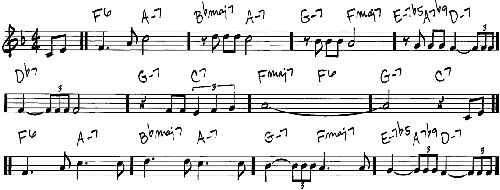
\includegraphics[width=10cm]{images/waww.jpg}
\caption{Lead sheet with the beginning of Louis Armstrong's \emph{What a wonderful world}\label{waww}}
\end{figure}

A \emph{chord} is a set of (at least three) notes; in this context it gives the current mood of the piece and jazz musicians can improvise the accompaniment of the melody with the notes of the chord. Chords are represented
\footnote{~~There are several ways of representing chords; this representation, the \emph{tabular notation}, is the most common in popular music (jazz, pop, rock\dots). But for instance, superposed notes on a classical music staff would also represent a chord.} 
by a letter from $A$ to $G$
\footnote{~~French equivalent: from \emph{la} to \emph{sol}.} 
with a possible \emph{accidental} ($\#$ for \emph{sharp}, $\flat$ for \emph{flat}, or nothing), representing the \emph{root note}, and a textual information giving the other notes relatively to the root note. For example, if we consider the $C\#m7$ chord (\guill{$C$ sharp minor seventh}), the notes will be the root note $C\#$, its \emph{minor third} $E$, its \emph{fifth} $G\#$ and its \emph{minor seventh} $B$. In jazz there are 313 possible such textual informations
\footnote{~~Actually, one could theoretically form different 56320 chords for a given root note; those 313 correspond to the \guill{harmonious} combinations, which is a subjective notion and thus depends on the music genre.}.

The dataset I worked on contains the lead sheets of 30 jazz pieces by famous artists like Louis Armstrong, Billie Holiday, Charlie Parker\dots~Some files describe the melodies as a sequence of notes (with pitch, onset and duration informations) and other contain the sequences of chords (sometimes with onset and duration informations). I did focus on the chord sequences with no timing information (as if for instance there was exactly one chord per bar). So, my data basically looked like:

\begin{equation*}
\text{\textbf{A Child Is Born:} } B\flat M7;~E\flat m;~B\flat M7;~E\flat m6;~B\flat M9;~E\flat m;~A~halfdim7;~D 7\#9\dots
\end{equation*}

I equally worked on the chord sequences of each song and on the concatenation of all the available sequences. This concatenation does not really make sense as a unique piece, but it is useful to do so in order to have an overview of all the corpus.

So, the motivation of my work was to provide an analysis of this data. The purpose of such an analysis is to gain knowledge about jazz and chord sequences, to understand it better, and also in a second time to use this knowledge to be able to compose similar music that would fit in the corpus.



\subsection{Chord similarities}

This section introduces the concept of chord similarity measures, and defines some measures from the state-of-the-art that I used.

\subsubsection{Introduction}

There are only 12 possible root notes because two notes separated by an \emph{octave} (concretely, whose frequencies ratio is a power of two) sound likewise, and are thus called the same: $C$ refers to low-pitched as well as to high-pitched sounds. The 12 notes correspond to a division of the octave into twelve equivalent \emph{semitones}; this is called the \guill{well-tempered} scale. 
So, as shown on figure \ref{keyboard}, the keyboard can be mapped to the cyclic group $\mathbb{Z}/12\mathbb{Z}$, and the notes to integers from $0$ to $11$.

\begin{figure}
\centering
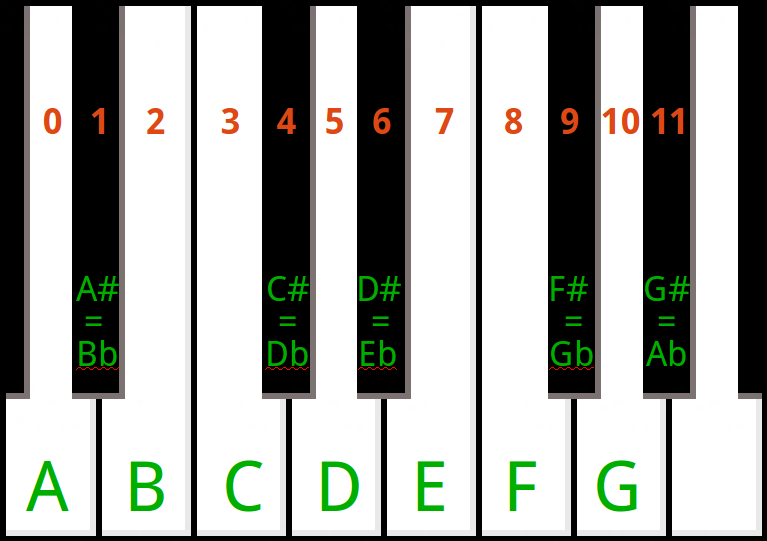
\includegraphics[width=6cm]{images/keyboard+.jpg}
\caption{A keyboard with notes names and their equivalent in $\mathbb{Z}/12\mathbb{Z}$\label{keyboard}}
\end{figure}

Then chords can be seen as subsets of $\mathbb{Z}/12\mathbb{Z}$. For instance, the previously seen $C\#m7$ chord would be mapped to the set $\{4;7;11;2\}$ (the order does not matter). Moreover the harmonic content in the chord name (here, \guill{$m7$}) can be seen as the vector and the root note (\guill{$C\#$}) as a starting point. Chords with same labels but different root notes are then the same by translation: $C\#m7$ corresponds to $\{4;7;11;2\}$ and $D\#m7$ to $\{5;8;12;3\}=\{4+1;7+1;11+1;2+1\}$.

It is hence possible to define mathematically distances between chord. However, such a distance much be chosen carefully to be relevant. Canonical distances do not necessarily mirror what is heard. With the $L_1$ distance (\guill{taxicab metric}) on chords of three notes, the chords $C=\{3;7;10\}$ and $Cm=\{3;6;10\}$ would be close since the difference is only of one semitone ($L_1(C,Cm)=1$); but to the ear they sound very different, one being major and the other minor. On the contrary, one would here something common between $C=\{3;7;10\}$ and $Bm=\{2;5;9\}$: they are \guill{inversions} of each other.


\subsubsection{Definitions of used measures}

In all, I used 9 different measures (in addition to the most simple one: equality), some rather elementary, some expressly developed by researchers. Three take as input the two chords to compare, $C_1$ and $C_2$, and return a boolean (\texttt{true} if and only if the chords are similar). All three define equivalence classes. They are:
\begin{itemize}
\item root note equivalence: \texttt{true} iff $C_1$ and $C_2$ have the same root note;
\item translational\footnote{~~\guill{translation} is the mathematical word; musicians would prefer \guill{transposition}.} 
equivalence: \texttt{true} iff $C_1$ and $C_2$ have the same harmonic indication (but possibly different root notes);
\item PCS-Prime equivalence (see \cite{forte}): \texttt{true} iff $C_1$ can be obtained from $C_2$ by a composition of inversions and translations;
\item 
\end{itemize}

The six other are distances\footnote{~~I use the word \guill{distance} to emphasize the difference with the first three measures; however all are not distances in a mathematical definition.}: they take as input two chords $C_1$ and $C_2$ and return a positive real number (all are scaled so that their image is $[0,1]$). As I will show in the next part, I did not need this value but to determine if to chord are \guill{close} of \guill{different}, so I used them with a threshold as additional input parameter. The measure will then return \texttt{true} if and only if the distance between $C_1$ and $C_2$ is greater than the threshold. They are:
\begin{itemize}
\item the F1-score;
\item Isaacson's similarity index, defined in \cite{isaacson};
\item Lewin's measure, defined in \cite{lewin};
\item Morris' measure, defined in \cite{morris};
\item Rahn's measure, defined in \cite{rahn};
\item Teitelbaum's measure, defined in \cite{teitelbaum}
\end{itemize}

The definitions of all these measures can be found in appendix. Here I will only present ???


\subsection{Compression algorithms}

The words \guill{analysis} and \guill{compression} will be used here with very close meanings. Indeed, compressing a piece means exhibiting its structure, separating the essential from the redundant. Hence, my analysis of the jazz lead sheets dataset will be described in terms of compression, and evaluated as such.

There are two complementary ways to approach computational music analysis
\footnote{~~They are of course also relevant in a wider context.}. 
One sees a piece as a linear sequence of notes (or chords, etc.), as the listener does: he can remember everything he heard but has no way to know what is coming until he actually hears it. The other views the piece from above, completely. Roughly, the first deals with linked lists and the second with arrays. It is the approach of Markov models \emph{versus} the one of formal grammars, Shannon's entropy \emph{versus} Kolmogorov's complexity.

My way of compressing simply describes a sequence of chords through the patterns (repeated sub-sequences) it contains, thus removing the redundancy. It is a closer to the second approach, and I developed it a lot more in this direction, but I implemented and tested algorithms for both, in order to be able to compare them. For the former, I used the classical algorithm known as LZ77; for the latter, what I called \guill{diagonal pattern decomposition}. They are presented in this order, after some basic definitions.


\subsubsection{Definitions}

The compressions are evaluated with their \emph{compression factor} and \emph{loss factor}.

The \emph{compression factor} corresponds to the size of the input data divided by the size of the compressed data. It is expected to be as high as possible (and at least greater than $1$). In here, it is considered that the size of a chord is the same as the size of an integer. Indeed, their are $7\cdot4\cdot313=6573$ possible chords, so a chord can be described with $\lceil log_2(6573)\rceil = 13$ bits; and the integer dealt with are lesser than $1469$ (the total number of chords in the database), thus defined by $\lceil log_2(6573)\rceil = 11$ bits. Of course, this definition fits the data I used and a different one could be needed for a different data.

There exist compression algorithms \emph{with} and \emph{without loss}. \emph{Without loss} means that the decompression of the compression is equal to the original sequence, while \emph{with loss} it is not necessarily so. The advantage of a compression with loss is that it can achieve better compression factors. I will define here the \emph{recovery factor} as the number of exact chords in the decompression of the compression of a piece, divided by the length of the piece. It is thus a real number between $0$ and $1$, that we will expect to be as close to $1$ as possible. This definition is rather sensitive; indeed, the loss will result of the use of similarity measures, and the original chords will be replaced during the compression by similar ones. However, the only other way to define would be to use precisely the similarity measure (\guill{the two corresponding chords are different by at most $x$ according to the measure}) but in my eyes not having an external evaluation would mean have too much faith in the measures; moreover one understands well what it is to be equal or different, but has no precise idea of what a difference of $x$ in a given measure could mean.


\subsubsection{Lempel-Ziv 77 (LZ77)}

The LZ77 algorithm, designed by A. Lempel and J. Ziv in 1977, introduced in \cite{lempelziv}, is a very popular compressing algorithm. It takes as input a list of data and outputs a list of triples of the form $(a,b,D)$ meaning \guill{go back $a$ times, copy the next $b$ data, and add $D$}. In the original algorithm, restrained buffer and preview size are given as parameters; however, I chose to let them be unbounded in order to focus on the best possible results. The obtained algorithm is given in \ref{algolz77}.

\begin{algorithm}
\setstretch{1.5}
\caption{LZ77 \label{algolz77}}
\SetKwData{iii}{i} \SetKwData{jjj}{j} \SetKwData{III}{I} \SetKwData{pref}{$\pi$} \SetKwData{aaa}{a} \SetKwData{bbb}{b} \SetKwData{buffer}{buffer} \SetKwData{LLL}{L}
\SetKwFunction{push}{push} \SetKwFunction{pop}{pop} \SetKwFunction{front}{front} \SetKwFunction{size}{size}

\KwIn{Queue of Chords $\III=(C_1, \dots, C_n)$.}
\KwOut{Queue of triples $\LLL=(a_j,b_j,C_{i_j})_j$.}

\Debut {
	\buffer $\leftarrow$ empty queue 

	\TantQue{\III is not empty} {
		\pref $\leftarrow$ longest prefix of \III in $(\buffer\cdot\III)$, beginning in \buffer

		\aaa $\leftarrow$ $\size(\buffer)$ $-$ (beginning index of \pref (in \buffer)) ($0$ if none)

		\bbb $\leftarrow$ length of \pref ($0$ if none)

		\Pour{\jjj \De $1$ \A \bbb} {
			$\buffer.\push(\front(\III))$

			$\III.\pop()$
		}
		$\LLL.\push(\aaa,\bbb,\front(\III))$

		$\buffer.\push(\front(\III))$

		$\III.\pop()$
	}
	\Retour \LLL
}
\end{algorithm}


For a better understanding, a complete example of an execution of the algorithm is given in appendix.

With a computation of the longest prefix in $\bigO{|\texttt{I}|^2}$, the overall complexity is $\bigO{|\texttt{I}|^3}$. There are better evaluations of this complexity but that are not of much interest here; knowing that it is polynomial and that the implementation runs fast is enough.

The LZ77 algorithm performs a compression without loss. I modified it in order to have a compression \emph{with loss}. The modification is very simple: when looking for the longest prefix, the algorithm will not only accept identical sequences, but also sequences that are similar up to a certain point. For a given measure $\mathfrak{M}$ and a threshold $t$ (let us assume that the image of $\mathfrak{M}$ is $[0,1]$ and that higher values correspond to more similar chords), two sequences $S_1$ and $S_2$ of the same length $n$ are considered similar if $\forall i \in [1,n], \mathfrak{M}(S_1[i],S_2[i]) \geq t$.


\subsubsection{Diagonal pattern decomposition}

My second approach uses \emph{diagonal patterns}. The best way to understand this notion is to visualise it. For a given piece, we write the chord sequence both vertically and horizontally. We can then consider a matrix whose cell $(i,j)$ will correspond to the $i$th and $j$th chords of the input sequence. Let us draw this cell in white if those chords are equal, and in black if they are different. We get a binary matrix on which  we can see the diagonal patterns, which are diagonal sequences of white cells. They correspond to sequence of chords that appear (at least) twice in the input piece, on two different positions. Such a matrix can be seen on figure \ref{diagonals}.

\begin{figure}
\centering
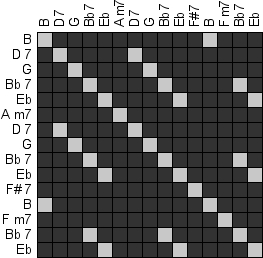
\includegraphics[width=6cm]{images/diagonals1.jpg}\hspace{1cm}
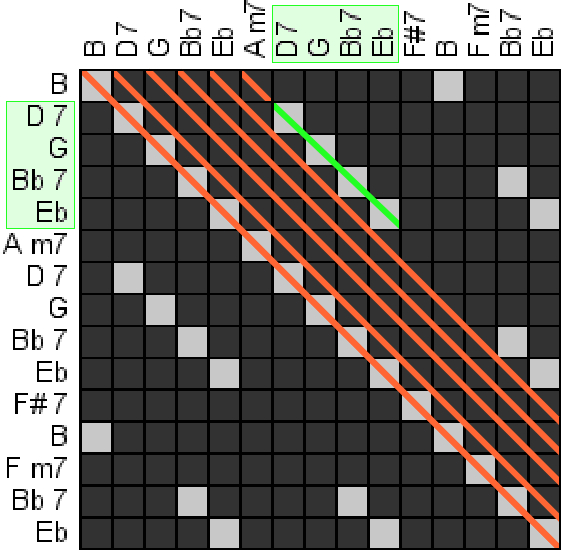
\includegraphics[width=6cm]{images/diagonals2.jpg}
\caption{A binary matrix and the diagonal search for patterns\label{diagonals}}
\end{figure}

A \emph{pattern} will then precisely be a maximal such sequence, along with its occurrences (positions where it occurs). \emph{Maximal} means that we consider only sequences having an occurrence that cannot be extended. Figure \ref{diagonals} shows the diagonal search for patterns and the maximal pattern $D7GB\flat 7E\flat$. $D7G$ is not maximal: every times it occurs it can be extended in the end. On the contrary, $B\flat 7E\flat$, which is included in $D7GB\flat 7E\flat$, is also a maximal pattern, occurring in the very end. In the piece of figure \ref{diagonals}, the diagonal patterns are (by increasing size):

\begin{itemize}
\item $B$, on positions 0 and 11;
\item $B\flat 7E\flat$, on positions 4, 8 and 13;
\item $D7GB\flat 7E\flat$, on positions 1 and 6.
\end{itemize}

As for the LZ77, I introduce here similarity measures, which will lead to a compression with loss. Instead of drawing a cell of the matrix in white only if the two corresponding chords are equal, this will be done also if they are similar for a given measure and up to a certain threshold. The matrix has then more white cells, implying more and longer patterns. Figure \ref{loose} shows this transformation (with the F1-score and a threshold of $0.9$).

\begin{figure}
\centering
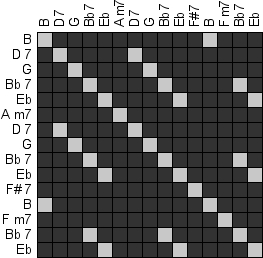
\includegraphics[width=6cm]{images/diagonals1.jpg}\hspace{1cm}
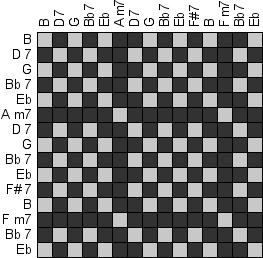
\includegraphics[width=6cm]{images/diagonals3.jpg}
\caption{Binary matrices for the same piece, the second using a similarity measure (F1 score)\label{loose}}
\end{figure}


Once the list of patterns established, the next step is to select a subset of these which is sufficient to describe the whole piece. In order to be sure this will always be possible (which is not the case in our example!), we add a \guill{pattern} for each single chord appearing in the piece (here: $(B;0,11)$, $(D7;1)$, $(G;2)$\dots). This subset should be as \guill{light} as possible, the \emph{weight} of a pattern being the sum of its length and of its number of occurrences. This problem is a \emph{weighted set cover}, which is NP-complete\footnote{~~See \href{https://en.wikipedia.org/wiki/Set\_cover\_problem}{https://en.wikipedia.org/wiki/Set\_cover\_problem} for more explanations on the set cover problem.}. So I implemented two heuristics, and the lighter results of the two will be selected. Briefly, their are both greedy algorithms; one aggregates patterns until covering the whole piece and the other removes as many patterns as possible from the exhaustive list. The pseudo-codes of these are given in the appendix.

For the decompression algorithm, the selected patterns are sorted by increasing number of occurrences and are copied in this order (so, a position that is covered by several patterns can be rewritten several times, and only the last, i.\!e. the corresponding chord of the pattern with most occurrences, will be kept). It is used to compute the \emph{recovery factor}. A pre-treatment is done on the patterns in order to maximize it (to minimize the loss). Indeed, a pattern occurring \emph{similarly} several times can correspond to several different exact sequences, and the recovery factor will depend on the choice of the sequence (which does not impact the compression factor) representing the pattern. For this, I simply compute for every pattern what positions of the reconstruction depend on it, and choose among the possible sequences the one that implies a minimum loss\footnote{~~This greedy algorithm, knowing the decompression scheme, is obviously optimal for this problem.}.

The complexity of the whole algorithm is $\bigO{|I|^5}$\footnote{~~See appendix for a brief analysis.}. This is quite high. In practice, the number of maximal patterns (which is $\bigO{|I|^2}$ in the worst case) seems to be the most determining factor for the running time. On my complete database (approximately 1500 chords), the execution takes between a few seconds and several minutes.


\subsection{Results}



\section{Other and further work}

\subsection{Grammatical inference}

\subsection{Segmentation}

\subsection{Improving the compression scheme}

PAPER

<=> MELODY

\subsection{The Lr2Cr8 project}



\section{Conclusion}





\section{Bibliography}
\nocite{*}

\bibliographystyle{plain}
\bibliography{mabiblio}




\end{document}


